%%%%%%%%%%%%%%%%%%%%%%%%%%%%%%%%%%%%%%%%%%%%%%%%%%%%%%%%%%%%%%%%%%%%%%
% How to use writeLaTeX: 
%
% You edit the source code here on the left, and the preview on the
% right shows you the result within a few seconds.
%
% Bookmark this page and share the URL with your co-authors. They can
% edit at the same time!
%
% You can upload figures, bibliographies, custom classes and
% styles using the files menu.
%
%%%%%%%%%%%%%%%%%%%%%%%%%%%%%%%%%%%%%%%%%%%%%%%%%%%%%%%%%%%%%%%%%%%%%%

\documentclass[12pt]{article}

\usepackage{sbc-template}
\usepackage[export]{adjustbox}
\usepackage{graphicx,url}

%\usepackage[brazil]{babel}   
\usepackage[utf8]{inputenc}  

     
\sloppy

\title{Tradutor Automatico para Língua Tupi}

\author{Rodemarck Júnior\inst{1},Tiago Barbosa de Lima\inst{1} Andre Nascimento\inst{1} }


\address{Departamento de Computação -- Universidade Federal Rural de Pernambuco
  (UFRPE)\\
  Rua Dom Manuel de Medeiros, s/n - Dois Irmãos, Recife - PE, 52171-900 Brazil
  \email{\{tiago.blima,rodemarck.meloj, andre.camara\}@ufrpe.br }
}

\begin{document} 

\maketitle
\begin{abstract}

    Recently neural networks are commonly used to several tasks, like the natural language processing having many applications, and one of them is the translation. Based on that, our project consists in make easier the access to the guarani, language of some Brazilians native speakers, which today has 5 thousand speaks, but it has no automatic translator available, like other native language like the Maori (language spoken for the New Zealand natives).
\end{abstract}

\begin{resumo}
Atualmente as redes neurais são comumente utilizados para diversas finalidades, como o processamento de linguagem natural tendo múltiplas aplicações, sendo a tradução uma delas. Baseado nisso, o projeto consiste em facilitar o acesso a guarani, idioma de nativos indígena que atualmente possui 5 mil falantes, porém não possui nenhum tradutor automático como já existem para língua faladas por nativos neozelandenses por exemplo.
\end{resumo}


\section{Introdução} 

~~~~~~~~~~O Brasil possui muitas riquezas culturais isso inclui a cultura indígena. O Brasil possui 305, dos 826 povos indígenas presentes na América latina \cite{povos_indigenas}. O tupi, ou tupi antigo era a língua falada pelas tribos de povos do grupo tupi, que habitavam a maior parte do litoral brasileiro \cite{Dicionario_Tupi_Antigo}.

O tupi antigo se tornou a língua franca do Brasil Colonia nos seculos XVI e XVII, quando os emigrantes portugueses e seus descendentes aprenderam e o difundiram, mais tarde as expedições bandeirantes levaram, antes restrito aos litorais, para todo o território brasileiro \cite{Tupi_Antigo}.

A língua tupi é sem duvida um de nossos muitos patrimônios culturais,  porém é uma língua com baixa acessionabilidade não existindo nenhum tradutor automático para o ela. O desenvolvimento de um tradutor poderia aumentar a acessibilidade a essa língua contribuindo para a preservação e difusão de tal patrimonio. 
%Acredito que não precisa ser explícito
%A motivação deste projeto é ajudar na preservação da língua tupi.

Na tentativa de criamos um tradutor nós implementamos um algoritmo de \textit{Deep Learning} que podem ser amplamente usados para construção de modelos de inteligência artificial capazes de prever resultados através de textos. No entanto ainda existente vários idiomas que não possuem tradução automática, como é o caso das línguas indígenas brasileiras, a qual são o objeto de estudo do projeto aqui apresentado.

\section{Tradução automática}
~~~~~~~~~~As línguas humanas consistem em morfologia (o modo com que as palavras são montadas a partir de pequenas unidades de sentido), sintaxe (o modo em que as frases são estruturadas) e semântica (o sentido das palavras e/ou frases).
A TA (tradução automática) é uma subseção da linguística computacional, é o processo automático de tradução de um idioma original para outro, através do uso de programas de computador. TA não é algo trivial, pois as línguas consistem mais de exceções do que de regras.

\section{Tradução por substituição}

~~~~~~~~~~O método mais simples de implementar um tradutor automático é dividir todas as palavras do texto, traduzir individualmente e substituir pelo texto original, pois tudo o que se precisa é um dicionario.

\subsection{Prós}

- Muito fácil de implementar.\newline
- Não exige muito processamento.

\subsection{Contras}

-Confiabilidade extremamente baixa, uma vez que ignora o contexto de cada palavra.\newline
-não leva em consideração a sintaxe da língua.

\section{Tradução por regras de sintaxe}

Primeiros sistemas de traduções automática, mais sofisticado que a tradução por substituição, pois depois de substituir as palavras por suas traduções aplicavam regras se sintaxe e semântica, para trocar as ordens das palavras adicionar conectivos, quando necessário, e as vezes até substituição da palavra por uma tradução que ofereça um resultado melhor.

\subsection{Prós}

- Leva em consideração o contexto e as regras de sintaxe\newline
- Pode ter regras adicionadas e atualizadas.\newline
- Tradução coerente e com boa confiabilidade para textos bem formatados e polidos.

\subsection{Contras}

- Custo extremamente elevado, pois cada língua possui milhares de regras próprias e com ainda mais exceções\newline
- Não consegue bons resultados se houver o menor desvio da linguagem culta.\newline
- Não leva em consideração o uso popular da língua.

\section{\textit{Statistical machine translation}}

~~~~~~~~~~A SMT (\textit{statistical machine translation}, ou máquina de tradução estatística) é uma abordagem diferente, que ao invés de regras de sintaxe usa estatística para traduzir e para isso utiliza uma grande de quantidade de textos possuindo a exata tradução para ambas as linguagens, essa coleção é chamada de corpora paralela. Esta foi a abordagem escolhida para este projeto.

Na SMT o textos não é dividido palavra a palavra, mas em trechos menores, mas que ainda possuam contextos. Em seguida é listado todas as possíveis traduções para cada, não apenas as que estão no dicionario, mas também lista traduções feitas por tradutores reais para aumentar as possibilidades de tradução, cada uma dessa possibilidades ganha uma pontuação baseada na frequência que essa tradução aparece. Milhares de combinações são geradas e a melhor tradução é escolhida baseada em sua pontuação e que seja considerada ``mais humana".

\subsection{Prós}

- Não fica restritos apenas as traduções do dicionário.\newline
- Leva em consideração o uso popular da língua.\newline
- Gera resultados que são mais facilmente entendidos.

\subsection{Contras}

- Necessita de grande base dados\newline
- Necessita de pré-processamento, pois precisa comparar verso a verso.

\section{Materiais}

~~~~~~O projeto utiliza palavras coletadas da tradução da Bíblia em Guarani disponível em \cite{angelo} e uma versão da Bíblia no idioma português Brasil na versão NTLH (Nova Tradução Linguagem de Hoje). A bíblia possui um imenso acervo de palavras (800 mil) se comparamos com outras literaturas similares \cite{Christodouloupoulos:2015:MPC:2767936.2767953}, além do fato que existem diversas traduções da bíblia segundo a \textit{United Bible Societies} existem 2,527 traduções parciais da bíblia e 475 completas \cite{Christodouloupoulos:2015:MPC:2767936.2767953}, sendo ideal para o processo de tradução. A bíblia também possui outra característica positiva como sua estrutura com versos bem definidos, sendo ideal para servir como corpora paralela.

Consideramos utilizar a  arquitetura de rede neural \textit{seq2seq}, esssa é amplamente utilizada para a geração de textos de traduções. Esse tipo de arquitetura é divida em duas partes o \textit{Encoder} que recebe a sentença a ser traduzida e o \textit{Decoder} que fornece a tradução, sendo portanto também conhecida como arquitetura \textit{Encoder}-\textit{Decoder} \cite{DBLP:journals/corr/ChoMGBSB14}. Tanto o \textit{Encoder} quanto o \textit{Decoder} são redes neurais recorrentes que a cada intereção tem o valor da saída atualizado por uma função de ativação \cite{DBLP:journals/corr/ChoMGBSB14}. Essas são treinadas juntas para maximizar a probabilidade de saída de um determinada tradução fazendo inicialmente um processo de pontuar cada par de versos utilizados.


Baseado nessa arquitetura foi  utilizado o algoritmo do \textit{tensorflow ``Translate with Attention"} disponível em \cite{tensorflow}. Nós também utilizamos a plataforma do Google colab \cite{google} para executarmos os teste.
Os arquivos foram coletados da bíblia (no formato .csv) do site \cite{angelo}, havendo um preprocessamento em que cada os versos eram alinhados tento em uma coluna com os versos em guarani e na outra em português.

\section{Métodos}

~~~~~~~Após a coleta e preprocessamento dos dados nós executamos 30 \textit{epoch} no nosso algoritmo com \textit{batch} de tamanho 64, dimensão 256 e unidades 1024. Nós começamos com 250 exemplos e aumentamos gradualmente a quantidade de exemplos até 1500 acrescentando a cada interação 250 exemplos usando 80\% para treino e 20\% para teste. Cada exemplo é representado por um par de palavras uma em português e a outra em Tupi que é repassada ao algoritmo para treinamento. Nossa abordagem utiliza o método desenvolvido por \cite{papineni2002bleu} para avaliação da traduções automáticas esse método utiliza uma lista com os candidatos e um outra lista com as referencias as quais são as traduções reais. Nesse método são comparados \textit{n-grams}
da tradução candidata com \textit{n-grams} da referência utilizado, onde \textit{n-grams} se entende por um conjunto de palavras ou frases adjacentes em um texto. Sendo assim, nós calculamos as médias das pontuações fornecida pela avaliação da tradução.

\subsection{Experimentos e Resultados}

No experimento cada verso está alinhado da seguinte forma:

\begin{center}
 \begin{tabular}{||c c c ||} 
 \hline
 1 & verso em guarani. & verso em português \\ [0.5ex] 
 \hline
 2 & verso em guarani & verso em português \\ 
 \hline
 3 & \vdots & \vdots  \\
 \hline
\end{tabular}
\end{center}

Após a leitura dos dados cada verso é colocado entre o $\langle\textit{START}\rangle$ e $\langle\textit{END}\rangle$ para indica o inicio e o fim do verso \cite{tensorflow}. Depois disso realizamos o processo de \textit{padding} para que ambos os versos tenham o mesmo tamanho e logo em seguida realizamos a criação dos \textit{tonkens} atribuindo a cada palavra em português e em guarani um valor numérico. Em seguida realizamos o processo de \textit{Encoder} para que possa ser a realizado o treinamento e \textit{Decoder} para transformarmos a saída em caracteres. Sendo assim nosso algoritmo irá ser treinado para aprender 

A imagem da figura 2 é proveniente de um resultado
de tradução da seguinte frase:
"No começo criou Deus os céus e a terra.".

Nós utilizamos a média do \textit{score} fornecido pelo método Bleu variando a quantidade de dados de teste obtendo diferentes pontuações para a precisão como mostrado no gráfico da figura 3.


\begin{figure}[h!]
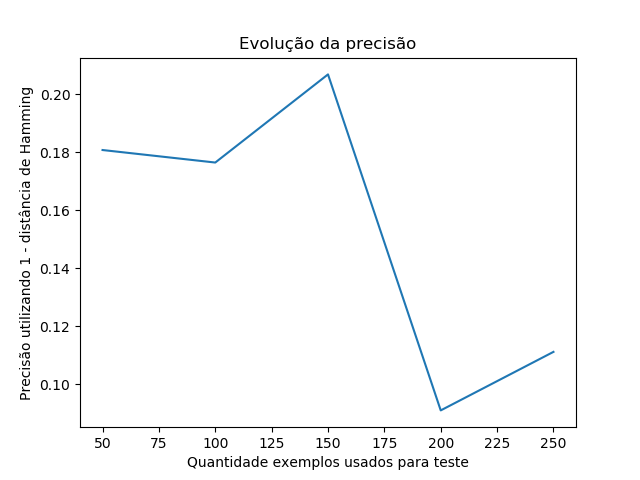
\includegraphics[width=.7\textwidth, center]{Figure_1.png}
\caption{Evolução da acurácia considerando exemplos de 250-1250 variando 250 a cada tentativa. }
\label{fig:figure1}
\end{figure}

\begin{figure}[h!]
\centering
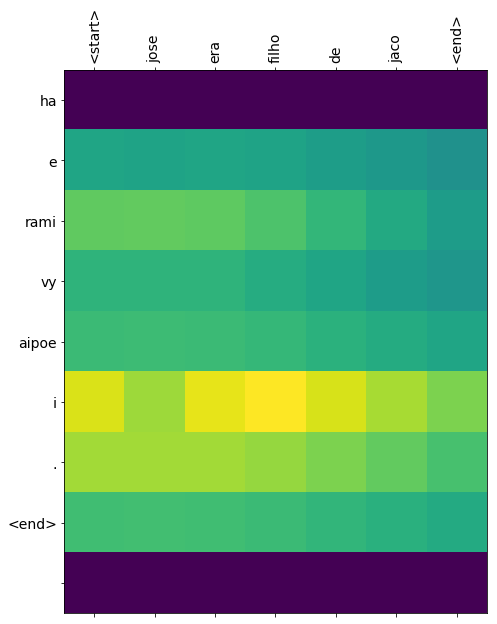
\includegraphics[width=.8\textwidth]{graph.png}
\caption{Resultado da tradução na última tentativa considerando 1500 exemplos, é mostrado as palavras levadas em conta com mais atenção na tradução. Obs.: Podem haver supressão de partes da tradução.}
\label{fig:exampleFig1}
\end{figure}



\section{Conclusão}\label{sec:figs}


Nosso tradutor ainda se encontrar no estado inicial precisando alguns modificações e aperfeiçoamentos apesar de já traduzir algumas palavras e frases do guarani para o português brasileiro. Além disso o algoritmo falha ao receber como entrar uma palavra não vista antes o, que pode ser melhorado usando técnicas de segmentação de cada palavra. Esperamos com o desenvolvimento desse projeto ajudar na preservação da cultura indígena e no divulgação de idiomas com essa origem.
\bibliographystyle{sbc}
\bibliography{sbc-template}

\end{document}
